\chapter{Omotopie: mappe tra cammini}
Concluso lo studio della topologia generale, vogliamo applicarla in un campo molto importante della matematica: la \textit{topologia algebrica}. \\ \\ Studieremo la struttura degli spazi (in particolare le superfici topologiche compatte): perché una tazza è un toro? per quale ragione una palla non è un toro? e soprattutto, a chi è venuto in mente di chiamare \enquote{toro} una ciambella?\\ Conosciamo la risposta all'ultima - gli antichi romani, deriva dal nome di un cuscino a forma di ciambella - ma per tutte le altre e molte di più addentriamoci nel mondo della topologia algebrica! \\ \\ In seguito riusciremo anche ad applicare le nuove strutture matematiche nella classificazione delle varietà.



\newpage
\section{Omotopie e retratti}
Cosa pensereste se qualcuno vi dicesse che può schiacciare una lattina rendendola un disco? Giochi da bambini, vero? \\ Beh, ora faremo la stessa cosa \dots ma con la matematica.
\subsection{\textcolor{TopAlg}{\textbf{Omotopie e classi di omotopia}}}
Vogliamo definire formalmente il concetto di \enquote{trasformare con continuità} due funzioni tra loro.

\begin{definition}
	Siano $\morphism{f_0, f_1}{X}{Y}$ mappe continue. Allora $f_0$ e $f_1$ si dicono \textbf{omotope} se esiste una funzione continua $\morphism{F}{X \times \left[0,1\right]}{Y}$ tale che $F(t,0) = f_0(t)$ per ogni $t \in X$ e $F(t,1) = f_1(t)$ per ogni $t \in X$.
\end{definition}

\begin{remark}[Omotopia come relazione di equivalenza]
	L'omotopia è una relazione di equivalenza.\\ Le prime due proprietà sono immediate, per la proprietà transitiva basta comporre le omotopie.
\end{remark}

\begin{definition}
	Siano $\morphism{f_0, f_1}{X}{Y}$ mappe continue e sia $A \subset X$. Allora $f_0$ e $f_1$ si dicono \textbf{omotope relativamente ad} $A$ se esiste una funzione continua $\morphism{F}{X \times \left[0,1\right]}{Y}$ tale che $F(t,0) = f_0(t)$ per ogni $t \in X$ e $F(t,1) = f_1(t)$ per ogni $t \in X$ e $F(a, t) = f_0(a) = f_1(a)$ per ogni $a \in A$.
\end{definition}

\begin{definition}
	Due spazi topologici $X,Y$ si dicono \textbf{omotopicamente equivalenti} se esistono le mappe continue $\morphism{f}{X}{Y}$, $\morphism{g}{Y}{X}$ tali che $g \circ f \sim \operatorname{Id}_X$ e $f \circ g \sim \operatorname{Id}_{Y}$. \\ In particolare si dice che \textit{sono nella stessa classe di omotopia} (o \textit{hanno la stessa classe di omotopia})
\end{definition}

\begin{remark}[Equivalenza omotopica]
	L'omotopia di spazi topologici è una relazione di equivalenza, si dimostra come in precedenza; non è difficile.
\end{remark}

\begin{remark}[Possibili fraintendimenti] Nonostante spesso e volentieri sia comodo pensare alla \enquote{deformazione continua} come una deformazione fisica dello spazio, è immediato verificare come \textbf{effettivamente non lo sia}. Notiamo che riferendoci agli spazi con \textit{deformazione continua} reciproca si intende il passaggio tra rappresentanti diversi della stessa classe di omotopia. \\ Si prenda una circonferenza con un punto esterno (spazio $A$) ed una circonferenza con un punto interno (spazio $B$), ovviamente sono nella stessa classe di omotopia. Però è impossibile deformarli \enquote{manualmente} fino ad ottenerli a vicenda, perché qualunque deformazione si compia prima o poi il punto interseca la circonferenza: in questo modo otterremmo uno spazio diverso sia da $A$ che da $B$, che non si trova neanche nella stessa classe di omotopia.
\end{remark}

\newpage
\subsection{\textcolor{TopAlg}{\textbf{Retratti e retratti di deformazione}}}

\begin{definition}
	Se $A \subset X$ dove $X$ spazio topologico allora $A$ è detto \textbf{retratto} di $X$ se esiste $\morphism{r}{X}{A}$ con $r$ continua e che $r(a) = a$ per ogni $a \in A$. In particolare $r \circ i_A = \operatorname{Id}_{A}$. \\ 
	In particolare	$A$ è detto \textbf{retratto di deformazione} di $X$ se è un retratto e $i_A \circ r \sim \operatorname{Id}_{X}$.\\ Ovviamente se è retratto di deformazione vuol dire che si trovano nella stessa classe di omotopia.
\end{definition}


\begin{remark}
	Alcuni esempi
	\begin{enumerate}
		\item Dimostriamo che $\R^n \setminus \{0\} \sim \S^{n-1}$. \\ Definiamo come retratto $\morphism{r}{\R^n \setminus \{0\}}{\S^{n-1}}$ con $r(x) = \frac{x}{\|x\|}$. Allora è ovvio che $r \circ i = \operatorname{Id}_{\S^{n-1}}$. Prendiamo quindi il caso $i \circ r = \frac{x}{\|x\|}$ con $x \in \R^n  \setminus \{0\}$. Dimostriamo che questa funzione è omotopa all'identità su $\R^n \setminus \{0\}$. Usiamo l'omotopia 
		\begin{equation*}
		F(s,t) = (1-t)(i \circ r) + tx
		\end{equation*} 
		ed abbiamo concluso.
		\item Definiamo ora la somma topologica di due spazi topologici $(X, \tau_1)$, $(Y, \tau_2)$ disgiunti. L'unione verrà definita come $(X \cup Y, \tau)$ dove $\tau$ è la topologia i cui aperti sono tali per cui $A \in \tau$ allora $A \cap X \in \tau_1$ e $A \cap Y \in \tau_2$. La somma topologica vera e propria $X \lor Y$ è definita come 
		\begin{equation*}
		X \lor Y := (X \cup Y, \tau) / \sim_{a_0, b_0}
		\end{equation*}
		dove $ a \sim_{a_0, b_0} b \iff a = b \lor (a = a_0 \land b = b_0)$. Ovvero unisce gli spazi e fa coincidere un punto dei rispettivi nello stesso. In pratica consideriamo il bouquet di due circonferenze $\S^1 \lor \S^1$ rappresentato in figura.
		
		\begin{figure}[h]
			\centering
			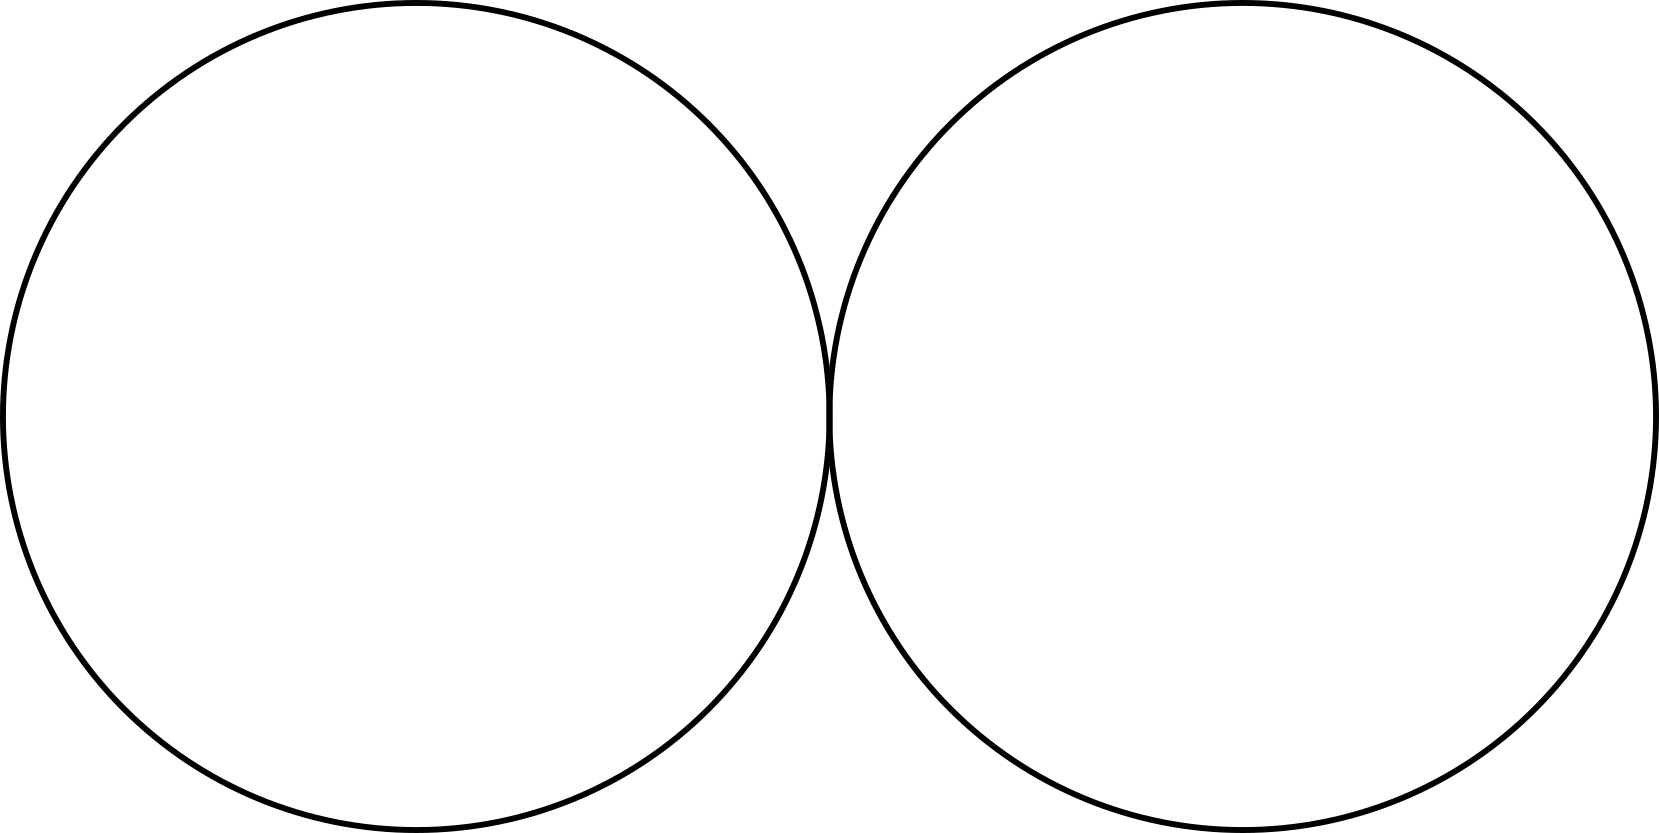
\includegraphics[width=0.3\linewidth]{images/topologia_algebrica/bouquet_circonferenze}
			\caption{}
			\label{fig:bouquetcirconferenze}
		\end{figure}
		Questo è ovviamente omotopo a $\R^2 \setminus \{(-1,0), (1,0)\}$ dove i punti scelti possono essere presi a piacere.
		\item Se $X \subset \R^n$ ed è un sottospazio stellato rispetto al centro $x_0$ allora $Y = \{x_0\}$ è un retratto di $X$. Infatti $X \sim \{p\}$ per qualsiasi $p \in \R^n$. Mostriamo intanto che $Y \sim X$. L'omotopia $F(x,t) = x - t(x-x_0)$ porta, in modo continuo, dalla funzione di $\morphism{id}{X}{X}$ (ovvero $x \mapsto x$) a $\morphism{i}{X}{X}$ (ovvero $x \mapsto x_0$). Ovvero $Y \sim X$.
		\item Sia $X = T$ toro. Allora $\morphism{r}{T}{\S^1}$ è un retratto su $\S^1 \subset T$, ma non è un retratto di deformazione. Infatti è impossibile trasformare (in modo continuo) un toro in una circonferenza. 
		\item Se si toglie un punto a il $g$-toro allora $T_g \setminus \{t\} \sim \underbrace{\S^1 \wedge \dots \wedge \S^1}_{2g-\text{volte}}$ 
		\item Analogamente per il piano proiettivo $U_h$, una volta tolto un suo punto ed ottenuto $U_h \setminus \{p\} \sim \underbrace{\S^1 \wedge \dots \wedge \S^1}_{h-\text{volte}}$
 	\end{enumerate}
\end{remark}

\newpage
\section{CW-complessi}
\subsection{\textcolor{TopAlg}{\textbf{Una semplice classe di spazi complessi}}}

Ora verranno introdotte delle classi di insiemi tali che possono essere suddivisi in parti \textit{retratte} e parti irriducibilmente non retratte, si veda il Teorema \ref{thr:contrai_ncelle_cw_complesso}.

\begin{definition}
	Uno spazio topologico $X$ si dice n-\textbf{cella} se $X \simeq \D^n$.
\end{definition}

\begin{definition}[Procedura di incollamento]
	\label{def:incollamento}
	L'incollamento di due spazi topologici $X,Y$ tramite $A \subset X$ è rapprensentato dal seguente diagramma
	\begin{equation*}
	\begin{tikzcd}
	A \arrow[d, hook]{i} \arrow[r]{f} & Y \\
	X
	\end{tikzcd}
	\end{equation*} 
	\begin{itemize}
		\item $f: A \to Y$ funzione \enquote{di incollamento}
		\item $i: A \to X$ inclusione
	\end{itemize}
	Lo spazio topologico risultante dall'incollamento è $X \sqcup Y / \sim$ dove usiamo la relazione $x \sim y \in Y \Longleftrightarrow x \in A \land f(x) = y$.
\end{definition}

\begin{remark}[Algoritmo di costruzione di un CW-complesso finito]
	$X$ è un CW-complesso se è possibile costruirlo secondo il seguente algoritmo:
	\begin{enumerate}
		\item Sia dato $X^0 \neq \varnothing$ insieme finito (detto anche $0$-scheletro)
		\item Sia $n \ge 1$, allora per ipotesi induttiva supponiamo di avere un $X^{n-1}$, ovvero un $(n-1)$-scheletro. Allora si incollano a $X^{n-1}$ delle $n$-celle attraverso il procedimento della Definizione \ref{def:incollamento} in cui vale 
		\begin{equation*}
		\begin{tikzcd}
			\S^{n-1} = \partial \D^n \arrow[d, hook]{i} \arrow[r]{f} & X^{n-1} \\
			\D^n
		\end{tikzcd}
		\end{equation*} 
		con $X^n = X^{n-1} \sqcup \D^n / \sim$ con la relazione specificata nella procedura di incollamento.
		\item Se il CW-complesso è di dimensione $N$, allora per $n = N$ il procedimento termina, con $X^N = X$.  
	\end{enumerate}
\end{remark}

\begin{definition}
	Sia $X$ un CW-complesso allora una \textbf{n-cella chiusa} in $X$ è l'immagine di $\morphism{f}{\D^n}{X}$ dove $f$ è definita come nella seguente successione
	\begin{equation*}
	\begin{tikzcd}
		\D^n \arrow[bend right=25, swap, hook]{rr}{f} \arrow[r,hook] & \D^n \sqcup X^{n-1} / \sim \arrow[r,hook] & X
	\end{tikzcd}
	\end{equation*}
\end{definition}

\begin{remark}
	In generale $\image{f} \neq \D^n$. Per esempio si prenda la costruzione di $\S^2$ come un CW-complesso con una $0$-cella e una $2$-cella che identifica tutto il suo bordo nel punto. Allora 
	\begin{equation*}
	\begin{tikzcd}
		\D^2 \arrow[bend right=25, swap, hook]{rr}{f} \arrow[r,hook] & \D^2 \sqcup \{p\} / \sim \arrow[r,hook] & \S^2
	\end{tikzcd}
	\end{equation*}
	è ovvio che $\image{f} = \S^2 \neq \D^2$. 
\end{remark}

\begin{definition}
	Sia $X$ un CW-complesso allora una n-cella aperta in $X$ è l'immagine di $\morphism{f}{\D^n}{X}$ dove $f$ è definita come nella seguente successione
	\begin{equation}
	\begin{tikzcd}
	\mathring{\D}^n \arrow[bend right=25, swap, hook]{rr}{f} \arrow[r,hook] & \mathring{\D}^n \sqcup X^{n-1} / \sim \arrow[r,hook] & X
	\end{tikzcd}
	\end{equation}
\end{definition}

\begin{remark}
	Le $n$-celle aperte sono omeomorfe al disco aperto $\mathring{\D}^n$. Infatti 
	\begin{equation*}
		\mathring{\D}^n \sqcup X^{n-1} / \sim\ = \mathring{\D}^n \sqcup X^{n-1}
	\end{equation*}
	poiché il bordo non dev'essere identificato (non fa parte dell'insieme $\mathring{\D}^n$).
\end{remark}

\begin{theorem}
	\label{thr:contrai_ncelle_cw_complesso}
	Se $X$ è un CW-complesso e $A \subset X$ è un sottocomplesso chiuso (ovvero un unione di $n$-celle chiuse) vale che se $A$ è contraibile allora $X$ è omotopo a $X / A$.
\end{theorem}
\begin{proof}
	Si può costruire la relazione di equivalenza utilizzando un po' di teoria dei grafi: sia data la foresta $F$ del grafo, intuitivamente si tratta del risultato della costruzione del CW-complesso una volta \enquote{elencati} i passaggi svolti su un diagramma ad albero. \\ Allora posso quozientare $X$ con la relazione di equivalenza
	\begin{equation*}
	x \sim y \iff \text{ hanno un albero in comune in $F$ }
	\end{equation*}
	La mappa quoziente $X \to X/\sim$ è una equivalenza omotopica. \\ Si noti inoltre che lo spazio quoziente eredita la struttura di CW-complesso. \\ \\ Ovviamente questa è solo un'idea di dimostrazione, la vera dimostrazione può essere svolta usando molta più teoria di algebra e sfruttando l'ipotesi di contraibilità (il modo in cui si usa è ovvio).
\end{proof}

I CW-complessi sono importanti poiché è possibile esprimere un invariante topologico. Infatti se due CW-complessi sono omeomorfi allora il valore della funzione caratteristica di Eulero è uguale. \\ Notiamo che usiamo i CW-complessi finiti perché sono compatti, e noi vogliamo classificare gli spazi compatti.

\begin{definition}
	Sia $X$ un CW-complesso costituito da $n_0$ $0$-celle, $\dots$, $n_N$ $N$-celle, allora 
	\begin{equation*}
		\chi(X) = \sum_{i=0}^{N} (-1)^i n_i
	\end{equation*}
	è la \textbf{funzione caratteristica di Eulero} di $X$. 
\end{definition}

\begin{remark}
	Alcuni esempi di CW-complessi
	\begin{enumerate}
		\item In generale un $g$-toro è composto da $1$ $0$-cella, $2g$ $1$-celle, $1$ $2$-cella. Quindi ha numero caratteristico $\chi(T_g) = 2(1-g)$. 
		\item In generale un piano proiettivo $U_h$ è composto da $1$ $0$-cella, $h$ $1$-celle, $1$ $2$-cella. Quindi ha numero caratteristico $\chi(U_h) = 2 - h$.
		\item Il disco $\D^n$ è una $n$-cella quindi $\chi(\D^n) = (-1)^n$. In generale il disco $n$-esimo si può costruire con una $0$-cella, una $(n-1)$-cella e $1$ $n$-cella.
	\end{enumerate}
\end{remark}

\begin{remark}
	Alcuni esempi del Teorema \ref{thr:contrai_ncelle_cw_complesso} possono essere i seguenti
	\begin{enumerate}
		\item Sia $X \subset \R^2$ come in figura 
		\begin{figure}[H]
			\centering
			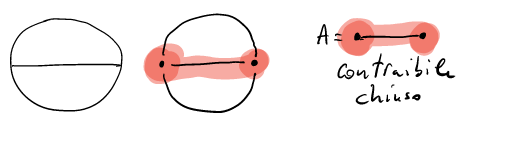
\includegraphics[width=0.6\linewidth]{images/topologia_algebrica/CWCOMPLEXEsempio1}
			\caption{}
			\label{fig:cwcomplexesempio1}
		\end{figure}
		allora è omotopicamente equivalente a un buquet di due circonferenze se si identifica la $1$-cella del diametro in un punto da cui
		\begin{figure}[H]
			\centering
			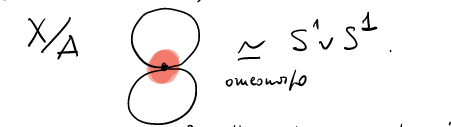
\includegraphics[width=0.6\linewidth]{images/topologia_algebrica/CWCOMPLEXEsempio2}
			\caption{}
			\label{fig:cwcomplexesempio2}
		\end{figure}
		\item Sia $X \subset \R^2$ come in figura 
			\begin{figure}[H]
				\centering
				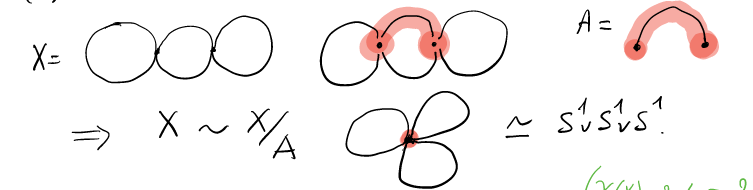
\includegraphics[width=0.7\linewidth]{images/topologia_algebrica/CWCOMPLEXEsempio3.png}
				\caption{}
				\label{fig:cwcomplexesempio3}
			\end{figure}
			identifichiamo una 1-cella della circonferenza centrale (l'insieme $A$) in un punto così da ottenere un bouquet di $3$ circonferenze per il Teorema \ref{thr:contrai_ncelle_cw_complesso}.   
		\item Sempre contraendo come in figura è abbastanza esplicito  che il grafo sia omotopo a un buquet di $4$ circonferenze.
			\begin{figure}[H]
				\centering
				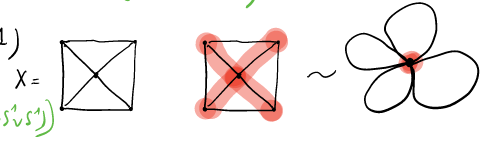
\includegraphics[width=0.7\linewidth]{images/topologia_algebrica/CWCOMPLEXEsempio8.png}
				\caption{}
				\label{fig:cwcomplexesempi4}
			\end{figure}
		\item Sia $X$ un toro con un disco e una circonferenza 
			\begin{figure}[H]
				\centering
				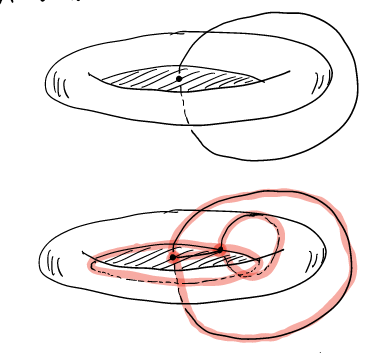
\includegraphics[width=0.3\linewidth]{images/topologia_algebrica/CWCOMPLEXEsempi4}
				\caption{}
				\label{fig:cwcomplexesempi4}
			\end{figure}
			Allora $X$ è un CW-complesso composto da $2$ $0$-celle, $4$ $1$-celle, $2$ $2$-celle. Posso contrarre il disco al centro del toro in un punto (perché possiamo è un retratto).   
			\begin{figure}[H]
				\centering
				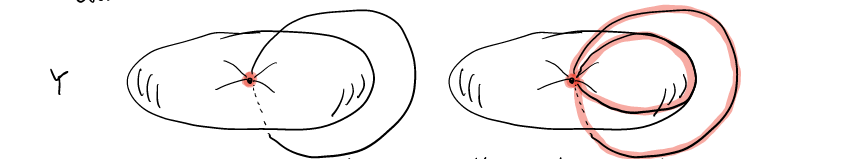
\includegraphics[width=0.7\linewidth]{images/topologia_algebrica/CWCOMPLEXEsempi5}
				\caption{}
				\label{fig:cwcomplexesempi4}
			\end{figure}
			Indichiamo con $Y$ l'insieme con il disco retratto in un punto. Poi \textit{allarghiamo} il toro in modo tale da ottenere una sfera con dentro parte della circonferenza identificata, otteniamo uno spazio omotopo allo spazio $Z$ come in figura
			\begin{figure}[H]
				\centering
				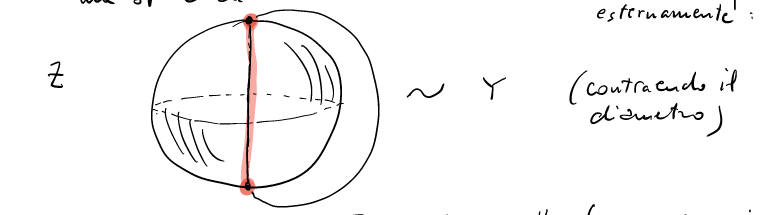
\includegraphics[width=0.7\linewidth]{images/topologia_algebrica/CWCOMPLEXEsempi6}
				\caption{}
				\label{fig:cwcomplexesempi4}
			\end{figure}
			e studiando $Z$ si ottiene uno spazio omotopicamente equivalente a $\S^2 \lor \S^1 \lor \S^1$
			\begin{figure}[H]
				\centering
				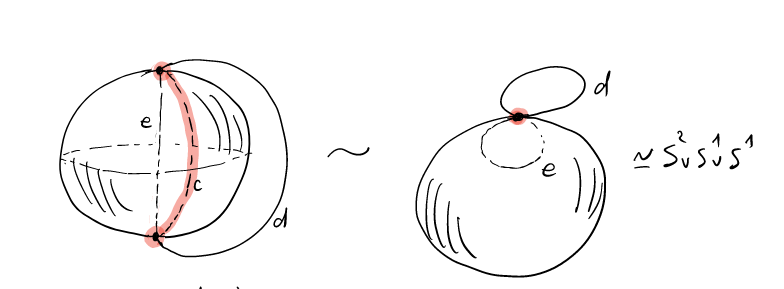
\includegraphics[width=0.7\linewidth]{images/topologia_algebrica/CWCOMPLEXEsempi7}
				\caption{}
				\label{fig:cwcomplexesempi4}
			\end{figure}
	\end{enumerate}
\end{remark}

\newpage
\section{Il gruppo fondamentale}
Esiste un gruppo che possiamo \enquote{incollare} ad uno spazio e che ne raccoglie le proprietà. In che senso \textit{ne raccoglie le proprietà}? \\ E soprattutto, come si costruisce? \\ Avendo struttura di gruppo è bene vedere alcuni teoremi puramente algebrici prima di continuare.
\subsection{\textcolor{TopAlg}{\textbf{Deformare cappi su una superficie}}}

\begin{definition}
	Sia $X$ spazio topologico, allora $\morphism{\alpha}{\left[0,1\right]}{X}$ tale che $\alpha(0) = x_0 \in X$ e $\alpha(1) = x_0 \in X$ con $\alpha$ continua si dice \textbf{cappio} di punto base $x_0$.
\end{definition}

\begin{definition}[Gruppo fondamentale] Sia $X$ uno spazio topologico, $x_0$ un punto appartenente ad $X$. Diciamo \textbf{gruppo fondamentale} di $X$ rispetto ad $x_0$ l'insieme delle classi di equivalenza omotopica dei cappi contenuti in $X$ con punto base $x_0$.
	\begin{equation*}
	\pi_1(X,x_0)= \left\{[\alpha] \ \big| \ \alpha \text{ è un cappio in $X$ di base $x_0$}\right\}
	\end{equation*}
	\begin{itemize}
		\item Uno spazio topologico $X$ si dice \textbf{semplicemente connesso} se $\pi_1(X, x_0) \simeq (\{1\}, +)$ ovvero il gruppo banale. 
	\end{itemize}
\end{definition}

\begin{definition}[Concatenazione di cammini]
	Definiamo l'operatore $*$ come la composizione delle classi omotopiche di cappi $\alpha, \beta$ (aventi estremi congiungibili) come segue
	\begin{equation*}
	\alpha * \beta :=
	\begin{cases}
		\alpha(2s) \quad 0 \le s \le 1/2 \\
		\beta(2s - 1) \quad 1/2 < s \le 1 \\ 
	\end{cases}
	\end{equation*}
\end{definition}

\begin{theorem}
	Siano $\alpha, \beta$ due cammini in $X$ tali che sia definito il prodotto e analogamente per i cammini $\gamma, \delta$. Allora se $\alpha \sim \gamma$ e $\beta \sim \delta$ vale $\alpha * \beta \sim \gamma * \delta$
\end{theorem}
\begin{proof} Basta scrivere l'omotopia: sia $F$ la prima e $G$ la seconda, l'omotopia cercata è
	\begin{equation*}
	H(s,t)=\begin{cases}
	F(2s,t) \ \ & 0 \leq s \leq \frac{1}{2}\\
	G(2s-1,t) \ \ & \frac{1}{2} \leq s \leq 1
	\end{cases}
	\end{equation*}
\end{proof}

\begin{theorem}
	$\pi_1(X, x_0)$ ha struttura di gruppo rispetto alla concatenazione di cammini. 
	\begin{equation*}
	(\pi_1(X, x_0), *) \ \text{è un gruppo}
	\end{equation*}
	In particolare, indicando con $x_k$ il cammino costante nel punto $x_k$ con un lieve abuso di notazione (altra notazione classica è $\varepsilon_{x_k}$), valgono
	\begin{enumerate}
		\item $x_0 * \alpha \sim \alpha \sim \alpha * x_1$
		\item $\alpha * \overline{\alpha} \sim x_0 \sim \overline{\alpha} * \alpha$.
		\item $(\alpha * \beta) * \gamma \sim \alpha * (\beta * \gamma)$
	\end{enumerate} 
\end{theorem}
\begin{proof} Verifichiamo intanto che riparametrizzando un cammino $\alpha$ non ne cambio la classe. Sia $\varphi:I \to I$ parametrizzazione continua, $\varphi(0)=0$ e $\varphi(1)=1$. La classe di omotopia non varia perché posso sempre scrivere l'omotopia
	\begin{equation*}
	F(s,t)=\alpha\big((1-t)s+t\varphi(s) \big)
	\end{equation*} 
	Allora posso dimostrare il teorema.
	\begin{enumerate}
		\item Basta trovare delle parametrizzazioni, la prima è
		\begin{equation*}
		\varphi(s)=
		\begin{cases}
		0 &  0 \leq s \leq \frac{1}{2}\\
		2s-1 &  \frac{1}{2} \leq s \leq 1\\
		\end{cases}
		\end{equation*}
		e la seconda 
		\begin{equation*}
		\varphi(s)=
		\begin{cases}
		2s  &  1 \leq s \leq \frac{1}{2}\\
		2s-1 &  \frac{1}{2} \leq s \leq 1\\
		\end{cases}
		\end{equation*}
		\item Trovare l'omotopia è banale, basta usare $\varepsilon_{x_0}$.
		\item Basta riparametrizzare in modo che
		\begin{equation*}
		(\alpha * \beta) * \gamma = \left((\alpha * \beta) * \gamma\right)\circ \varphi \sim \alpha * (\beta * \gamma)
		\end{equation*}
	\end{enumerate}
\end{proof}

\begin{theorem}
	Sia $X$ spazio topologico tale che $x_0 \in X$ è connesso per archi ad $x_1 \in X$, allora $\pi_1(X, x_0) \simeq \pi_1(X, x_1)$
\end{theorem}
\begin{proof} Sia $f$ l'arco congiungente i due punti, usiamo $u_f$ funzione tra i due gruppi fondamentali tale che
	\begin{equation*}
	u_f\left([\alpha]\right)=[(\overline{f}*\alpha)*f]
	\end{equation*}
	\begin{itemize}
		\item \textbf{Ben definita}\\
		Se $a \sim b$ allora $f*a \sim f*b$ e $(\overline{f}*a)*f=(\overline{f}*b)*f $ per quanto appena dimostrato.
		\item \textbf{Omomorfismo di gruppi}
		\begin{align*}
		u_f\left([a][b]\right)& =u_f\left([a*b]\right)=\left[\left(\overline{f}*(a*b)\right)*f\right]
		\end{align*}
		\begin{align*}
		u_f([a])\cdot u_f([b]) & = \dots \\
		& = \left[\left((\overline{f}*a)*f\right)*\left((\overline{f}*b)*f\right)\right]\\
		& = \left[\left(\overline{f}*\left((a*f)*(\overline{f}*b)\right)\right)*f\right]\\
		& = \left[\left(\overline{f}*(a*b)\right)*f\right]
		\end{align*}
		\item \textbf{Isomorfismo di gruppi}\\
		Ovvio, basta usare $u_{\overline{f}}$.
	\end{itemize}
\end{proof}

\begin{corollary}
	Se $X$ è connesso per archi allora il suo gruppo fondamentale è unico al più per isomorfismi.
\end{corollary}

\begin{proof} Particolarmente ovvio, inclusa solo per completezza; se lo spazio è connesso per archi vuol dire che la componente connessa per archi più grande è lo spazio stesso e per teorema esiste un arco tra ogni punto scelto a piacere verso ogni altro punto.
\end{proof}	
	
\begin{theorem}
	Sia $\morphism{\varphi}{X}{Y}$ una mappa continua tra spazi topologici, allora induce un omomorfismo tra i relativi gruppi fondamentali 
	\begin{align*}
	\varphi_*:\pi_1(X, x_0)&\to\pi_1(Y, \varphi(x_0))\\
	[\alpha] &\to [\varphi \circ \alpha]
	\end{align*}
	Inoltre l'operatore $_*$ gode delle \textit{proprietà funtoriali}:
	\begin{enumerate}
		\item $(\varphi \circ \psi)_* = \varphi_* \circ \psi_*$
		\item $(\operatorname{Id}_{X})_* = \operatorname{Id}_{\pi_1(X, x_0)}$ 
	\end{enumerate}
\end{theorem}
\begin{proof} Osserviamo che il morfismo indotto è ben definito.  
	\begin{equation*}
	a \sim b \implies \varphi\circ a \sim \varphi\circ b
	\end{equation*}
	infatti data $F$ prima omotopia basta usare $G=\varphi\circ F$. Risulta immediato anche dimostrare che è effettivamente un morfismo di gruppi, basta notare che $\varphi\circ(a*b)=(\varphi\circ a)*(\varphi\circ b)$.
\end{proof}

\begin{corollary}
	Se $\morphism{\varphi}{X}{Y}$ è un omeomorfismo di spazi topologici allora $\varphi_*$ è un isomorfismo di gruppi. In particolare il gruppo fondamentale è un \textit{invariante topologico}.
\end{corollary}

\begin{proof}
	Sia $f$ funzione continua che induce il morfismo $f_*$. \\ Allora per $x\in X$:
	\begin{align*}
	\left(f^{-1}\right)_*\circ f_* = \left(f^{-1}\circ f_*\right)=\operatorname{Id}_{\pi({X,x})}
	\end{align*}
	\begin{align*}
	f_*\circ\left(f^{-1}\right)_*  = \left(f_*\circ f^{-1} \right)=\operatorname{Id}_{\pi({Y,f(x)})}
	\end{align*}
\end{proof}

\begin{theorem}
	Se $A \subset X$ è un retratto di $X$ con $r$ come retrazione, allora vale che $\pi_1(A, x_0) \subset \pi_1(X, x_0)$ ed è un sottogruppo.  \\ In particolare $r_*\circ i_* =\operatorname{Id}_{\pi_{A,a}}$.
\end{theorem}
	\begin{proof}Particolarmente ovvio, basta scrivere:
		\begin{equation*}
		r_*\circ i_* =(r\circ i)_* = (\operatorname{Id}_{A})_*=\operatorname{Id}_{\pi({A,a})}
		\end{equation*}
		Per ogni retratto $A$ inoltre $i_*$ è un isomorfismo del suo gruppo fondamentale con immagine un sottogruppo di $\pi(X,a)$.
	\end{proof}

\subsection{\textcolor{TopAlg}{\textbf{Il teorema di invarianza omotopica}}}
Vogliamo dimostrare un risultato potente: il gruppo fondamentale è invariante omotopico. Per farlo dobbiamo sviluppare ulteriormente la teoria.
\begin{lemma}
	Siano $\Phi$ e $\Psi$ funzioni continue ed omotope tra $X$ ed $Y$, $F$ loro omotopia. Sia $f(t)=F(x_0,t)$ cammino tra $\Phi(x_0)$ e $\Psi(x_0)$. Allora il seguente diagramma commuta (questo vuol dire che $\Phi_*=u_f\circ \Phi_*$).
	\begin{equation*}
	% https://tikzcd.yichuanshen.de/#N4Igdg9gJgpgziAXAbVABwnAlgFyxMJZABgBpiBdUkANwEMAbAVxiRAB120sAKADVIAPAPrEAlCAC+pdJlz5CKAEzkqtRizaduPAJqlOABQAWvEeInTZ2PASIBGUvbX1mrRBy699R7D3NilmowUADm8ESgAGYAThAAtkhkIDgQSCogDHQARjAMhnK2iiBYYNiwINSumh6+WMIAVFIyILEJSdSpSI6ZOXkFNgpspeWsVRrunib1TVatcYmIPV2IGVm5+YVDHiNYFeNubEzCUVIUkkA
	\begin{tikzcd}
	{\pi(X,x_0)} \arrow[rd, "\Psi_*" description] \arrow[rr, "\Phi_*" description] &                    & {\pi(Y,\Phi(x_0))} \arrow[ld, "u_f" description] \\
	& {\pi(Y,\Psi(x_0))} &                                                 
	\end{tikzcd}
	\end{equation*}
\end{lemma}
\begin{proof} Devo mostrare che per ogni $A=[a]\in\pi(X,x_0)$ vale 
	\begin{align*}
	(u_f\circ \Phi_*)(A) &= [(\overline{f}*(\Phi\circ a))*f] \\
	&=[\Psi\circ a]=\Psi_*(A)
	\end{align*}
	(cioè che $(\overline{f}*(\Phi\circ a))*f \sim \Psi\circ a$) \\ 
	Sia $y_0=\Phi(x_0)$, so che $\Psi\circ a \sim (\varepsilon_{y_0}*(\Phi \circ a))*\varepsilon_{y_0}$. Ho risotto la tesi a 
	\begin{equation*}
	(\overline{f}*(\Phi\circ a))\sim (\varepsilon_{y_0}*(\Phi \circ a))*\varepsilon_{y_0}
	\end{equation*}
	Ricordo che $f$ è un cammino da $\Phi(x_0)$ ad $y_0$, allora 
	\begin{enumerate}
		\item $\overline{f}\sim \varepsilon_{y_0}$ tramite $\overline{G}(s,t)=f\left((1-t)s\right)$
		\item $f\sim \varepsilon_{y_0}$ tramite $\overline{G}(s,t)=f\left((1-t)s+t\right)$
		\item $\Phi*a \sim \Psi*a$ tramite $K(s,t)=F\left(a(4s-1),t\right)$
	\end{enumerate}
	Allora posso dimostrare la tesi riparametrizzando.
	\begin{equation*} 
	H(s,t)=
	\begin{cases}
	\overline{G}(4s,t)=\overline{f}\left((1-t)4s\right) & s \in [0,\frac{1}{4}]\\
	K(4s-1,t)=F\left(a(4s-1),t\right) & s \in [\frac{1}{4},\frac{1}{2}]\\
	G(2s-1,t)=f\left((1-t)(2s-1)+t\right) & s \in [\frac{1}{2},1]
	\end{cases}
	\end{equation*}
	ed ovviamente è continua perché per ogni $t \in [0,1]$ le definizioni coincidono.
\end{proof}

\begin{corollary}[Teorema di invarianza omotopica] Siano $X$ ed $Y$ spazi con $\varphi$ omotopia equivalenza omotopica. Allora il suo morfismo indotto tra i gruppi fondamentali è un isomorfismo.
\end{corollary}
\begin{proof} Sia $y=\varphi(x)$, sia $\psi$ l'altra equivalenza omotopica. Allora sappiamo che 
	\begin{enumerate}
		\item 	$\psi \circ \varphi \sim \operatorname{id}_X$
		\item	$\varphi \circ \psi \sim \operatorname{id}_Y$ 
	\end{enumerate}
Inoltre dico $\Phi$ l'identità in $X$ e $\Phi$ $\psi \circ \varphi$.
	\begin{equation*}
	% https://tikzcd.yichuanshen.de/#N4Igdg9gJgpgziAXAbVABwnAlgFyxMJZABgBpiBdUkANwEMAbAVxiRAB120sAKADVIAPAJQgAvqXSZc+QigCMpeVVqMWbTt35DREqdjwEiAJnIr6zVog5deAzgAUAFrwCew3ZJAYDsoospqC3VrTV4ATVJ3cRUYKABzeCJQADMAJwgAWyQAZmocCCRTEAY6ACMYBgdpQzkQLDBsWBAgtSsbNGwAfQAqcS90rKQyEAKkRRLyyurfI2sGptZWyw12CDQYNLoCtLA6TJhgLCgxLuAw7RExftSM7MRiscQJ0oqqmr95xuOl1RXrJhdFI3ECDe4jJ55SZvGYyOb1b7NZYhGz0NJoFy9GJiIA
	\begin{tikzcd}
	{\pi(X,x)} \arrow[rd, "{\operatorname{id}_{\pi(X,x)}}" description] \arrow[r, "\varphi_*" description] & {\pi(Y,y)} \arrow[r, "\psi_*" description] & {\pi(X,\Phi(y))} \arrow[ld, "u_f" description] \\
	& {\pi(X,x)}                                 &                                               
	\end{tikzcd}
	\end{equation*}
	$u_f$ è l'isomorfismo relativo al cambio di punto base, siccome vale che 
	\begin{equation*}
	u_f \circ \psi_* \circ \phi_* = \operatorname{id}_{\pi(X,x)}
	\end{equation*}
	allora abbiamo che $\psi_* \circ \phi_*$ è un isomorfismo, quindi $\psi_*$ è suriettiva e $\phi_*$ iniettiva. Posso applicare il lemma alla funzione $\varphi \circ \psi \sim \operatorname{id}_Y$, ottengo il seguente diagramma commutativo.
	\begin{equation*}
	% https://tikzcd.yichuanshen.de/#N4Igdg9gJgpgziAXAbVABwnAlgFyxMJZABgBpiBdUkANwEMAbAVxiRAB120sAKATVIBPAJQgAvqXSZc+QigCM5KrUYs2nbjwAapDdh4jREqdjwEiAJiXV6zVog5csnBjABmOfrq4ALXnt5DTgAnLABzHxxhI0kQDFNZIkV5ZVs1Bw1eARFxZRgoMPgiUDdgiABbJDIQHAgkAGYbVXtHCDQYYLpa4LA6cphgLCgxAH1gTK8RMRBqBjoAIxgGAAVpMzkQLDBsWHFY0oqq6lqkRRU7dS5sEYAqGZA5xZW1xIctndZjEAPKxGqTxBWc7pEA8DR+TgAYywwUhAWEt3ujyWqwS5je2yGrGoizAUAaxC+P1OxzqgKaFwy7DwDFg43Y9GCaD8ozuswWKJe6M2mN2RLKvyBAMawJaTBGYSRHOeaI27yxuTEQA
	\begin{tikzcd}
	{\pi(Y,y)} \arrow[rd, "{\operatorname{id}_{\pi(Y,y)}}" description] \arrow[r, "\psi_*" description] \arrow[rr, "(\phi\circ\psi)_*" description, bend left] & {\pi(X,\psi(y))} \arrow[r, "\tilde{\varphi}_*" description] & {\pi\left(Y,\phi(\psi(y))\right))} \arrow[ld, "u_g" description] \\
	& {\pi(Y,y)}                                                  &                                                                 
	\end{tikzcd}
	\end{equation*}
	Siccome $u_g$ è un isomorfismo, $\tilde{\varphi}_*$ è un isomorfismo indotto da $\varphi$ (in generale diverso da $\varphi_*$ perché dipende dal punto base scelto, qui il punto base è $phi(y)$ generalmente diverso da $x$). Allo stesso modo di prima ottengo che $\tilde{\varphi}_*\circ\psi_* $ è un isomorfismo di gruppi, quindi $\psi_*$ è iniettiva.
\end{proof}





\section{Il teorema di Seifert-van Kampen}
\subsection{\textcolor{TopAlg}{\textbf{Enunciato e conseguenze}}}


\begin{theorem}[Teorema di Seifert-van Kampen]
	Dati due aperti $U, V$ tali che $U \cap V \neq \varnothing$ e tutti gli insiemi sono connessi per archi, allora se $X = V \cup U$ e $x_0 \in U\cap V$ segue che 
	\begin{equation*}
		\pi_1(X, x_0) \simeq \pi_1(H, h_0)
	\end{equation*} 
	dove 
	\begin{equation*}
	\pi_1(H,h_0) = \left\langle U \cup V \mid R_1 \cup R_2 \cup R_S \right\rangle
	\end{equation*}
	\begin{equation*}
	R_S := \{s \in \pi_1(U \cap V,x_0) \mid (i^{-1}_V \circ i_{U}) \left[s\right] = \left[s\right]\}
	\end{equation*}
\end{theorem}
%\begin{proof}
	% TODO
%\end{proof}

\begin{theorem}
	Sia $x_0$ il punto $(1,0) \in S^1$ allora $\pi_1(S_1, x_0) \simeq \Z$.
\end{theorem}



\subsection{\textcolor{TopAlg}{\textbf{Applicazioni di Seifert-van Kampen}}}
Presento alcuni corollari utili allo svolgimento degli esempi successivi.

\begin{corollary}
	Siano $U,V$ aperti e semplicemente connessi, allora se $U \cap V$ è connesso per archi vale $\pi_1(U\cup V,x_0) \simeq \Z_1$ 
\end{corollary}

\begin{corollary}
	Siano $U,V$ aperti tali e tali che $U \cap V$ è connesso per archi e contraibile, allora $\pi_1(U \cup V, x_0) \simeq \left\langle U \cup V \mid R_U \cup R_V\right\rangle$.
\end{corollary}


\begin{xca}
	Per $n \ge 2$ le $n$-sfere hanno gruppo fondamentale banale. \\ Ovvero $\pi_1(S^n, x_0) \simeq \Z_1$
\end{xca}
\begin{proof}
	Considero $U,V$ rispettivamente come l'emisfero nord e l'emisfero sud. Allora questi sono aperti e hanno $U \cap V \simeq S^{n-1}$. Siccome $U, V$ sono semplicemente connessi (sono omeomorfi a un disco), vale il corollario precedente e dunque $S^n$ è semplicemente connesso.  
\end{proof}

\begin{xca}
	Sia $\S^1 \lor \dots \lor \S^1$ il bouquet di $n$-circonferenze. \\ Allora $\pi_1(\S^1 \lor \dots \lor \S^1, x_0) \simeq \Z \ast \dots \ast \Z$
\end{xca}
\begin{proof}
	Dimostriamo nel caso $n=2$ poiché la dimostrazione è la medesima per ogni $n \ge 2$. Prendiamo come $U, V$ le due circonferenze più un po' dell'altra aventi come intersezione $U \cap V$ che contiene il punto di incollamento e un po' delle due circonferenze (si veda figura). In questo modo $U,V,U \cap V$ sono aperti e connessi per archi.
	% TODO: \usepackage{graphicx} required
	\begin{figure}[h]
		\centering
		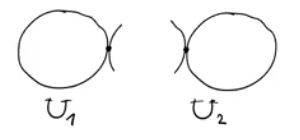
\includegraphics[width=0.4\linewidth]{images/topologia_algebrica/bouquet-circle-fundamental-group}
		\caption{}
		\label{fig:bouquet-circle-fundamental-group}
	\end{figure}
	Possiamo usare il teorema dei CW-complessi per ritrarre $U \sim \S^1$ e $V \sim \S^1$, mentre l'intersezione è ritraibile in un punto. Quindi diventa che 
	\begin{equation*}
		\pi_1(\S^1 \lor \S^1, x_0) \simeq \left\langle \alpha, \beta \mid \varnothing \right\rangle \simeq \Z \ast \Z
	\end{equation*}
\end{proof}

\begin{xca}
	Dimostriamo il seguente isomorfismo $\pi_1(T_1, x_0) \simeq \Z^2$
\end{xca}
\begin{proof}
	Prendiamo come suddivisione del toro gli aperti $U_1, U_2$ dove $U_1$ è il toro tolto un punto $Q$, mentre $U_2$ è il toro tolto i lati perimetrici che vengono incollati per costruire il toro (si veda la figura)
	\begin{figure}[h]
		\centering
		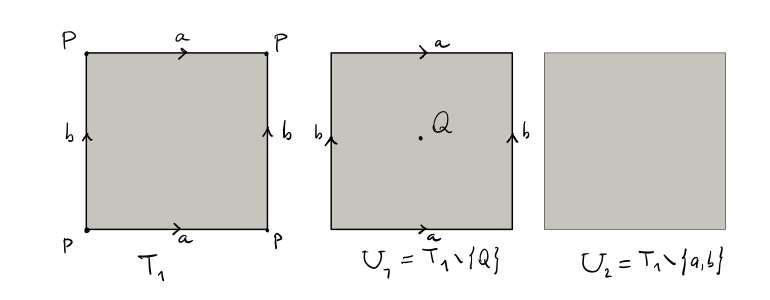
\includegraphics[width=0.7\linewidth]{images/topologia_algebrica/fundamental-group-torus}
		\caption{}
		\label{fig:fundamental-group-torus}
	\end{figure}
	Allora sappiamo che $\pi_1(U_1,x_0) \simeq \pi_1(\S^1 \lor \S^1, x_0) \simeq \Z \ast \Z$, mentre $U_2$ è contraibile (è essenzialmente un disco aperto). L'intersezione $U_1 \cap U_2$ invece è omotopicamente equivalente a $\S^1$, infatti se il buco si può allargare fino ad ottenere $\S^1$. Per cui otteniamo i seguenti risultati
	\begin{align*}
		\pi_1(U_1) & \simeq \Z \ast \Z \\
		\pi_1(U_2) & \simeq \Z_1 \\
		\pi_1(U_1 \cap U_2) &\simeq \Z \\
	\end{align*}
	poiché $\pi_1(U_1 \cap U_2)$ non è banale dobbiamo vedere quale è la relazione $R_{U_1 \cap U_2}$. Per vedere come interagisce sui cappi, dobbiamo ossservare che ogni cappio $c \in \pi_1(U_1 \cap U_2)$ può essere portato sul bordo di $U_1$ e, ciascuno dei cappi $c$ percorre i lati del toro in senso $aba^{-1}b^{-1}$, questo coincide alla relazione sui cappi di $\pi_1(U_1)$: $a \ast b \ast a^{-1} \ast b^{-1} = 1$ (si veda figura)
	\begin{figure}[h]
		\centering
		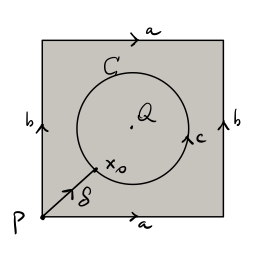
\includegraphics[width=0.4\linewidth]{images/topologia_algebrica/fundamental-group-torus-2}
		\caption{}
		\label{fig:fundamental-group-torus-2}
	\end{figure}	
	per cui diventa
	\begin{equation*}
		\pi_1(U_1 \cup U_2, x_0) \simeq \left\langle \{\alpha, \beta\} \cup \varnothing \mid R_{U_1 \cap U_2} \right\rangle \simeq \left\langle \alpha, \beta \mid \alpha \beta = \beta \alpha \right\rangle \simeq \Z^2
	\end{equation*} 
\end{proof}

\begin{xca}
	Dimostrare per ragionamento analogo a quello del toro che 
	
	\begin{equation*}
		\pi_1(U_h, x_0) \simeq \left\langle \alpha_1, \dots, \alpha_h \mid \alpha^2_1 \cdots \alpha^2_h = 1\right\rangle
	\end{equation*}.
\end{xca}
\begin{proof} Versione breve: \\
	Lo spazio proiettivo reale $U_1$ si costruisce come disco chiuso con due archi di circonferenza identificati. Prendo $V_1$ e $V_2$ esattamente come nel toro:
	\begin{itemize}
		\item $V_1$ è un bouquet di una circonferenza, di generatore $\alpha$
		\item $V_2$ è contraibile
		\item L'intersezione si retrae con deformazione su una circonferenza, dico $\delta$ il generatore di questa circonferenza
	\end{itemize}
	Siccome sono connessi per archi posso ragionare come sempre con il teorema di van Kampen ed ottengo (dato $sigma$ il solito cammino):
	\begin{equation*}
	[\delta]=\begin{cases}
	[\sigma \alpha^2 \sigma^{-1}]=[\sigma \alpha \sigma^{-1}]^2=A^2 & \text{ in $V_1$}\\
	1 & \text{ in $V_2$}
	\end{cases}
	\end{equation*}
	Quindi si vede che il gruppo fondamentale dello spazio proiettivo reale ha forma
	\begin{equation*}
	\pi(U_1,x)=\left\langle A \ | A^2 = 1 \right\rangle 
	\end{equation*}
\end{proof}
